% Options for packages loaded elsewhere
\PassOptionsToPackage{unicode}{hyperref}
\PassOptionsToPackage{hyphens}{url}
%
\documentclass[
]{book}
\usepackage{lmodern}
\usepackage{amsmath}
\usepackage{ifxetex,ifluatex}
\ifnum 0\ifxetex 1\fi\ifluatex 1\fi=0 % if pdftex
  \usepackage[T1]{fontenc}
  \usepackage[utf8]{inputenc}
  \usepackage{textcomp} % provide euro and other symbols
  \usepackage{amssymb}
\else % if luatex or xetex
  \usepackage{unicode-math}
  \defaultfontfeatures{Scale=MatchLowercase}
  \defaultfontfeatures[\rmfamily]{Ligatures=TeX,Scale=1}
\fi
% Use upquote if available, for straight quotes in verbatim environments
\IfFileExists{upquote.sty}{\usepackage{upquote}}{}
\IfFileExists{microtype.sty}{% use microtype if available
  \usepackage[]{microtype}
  \UseMicrotypeSet[protrusion]{basicmath} % disable protrusion for tt fonts
}{}
\makeatletter
\@ifundefined{KOMAClassName}{% if non-KOMA class
  \IfFileExists{parskip.sty}{%
    \usepackage{parskip}
  }{% else
    \setlength{\parindent}{0pt}
    \setlength{\parskip}{6pt plus 2pt minus 1pt}}
}{% if KOMA class
  \KOMAoptions{parskip=half}}
\makeatother
\usepackage{xcolor}
\IfFileExists{xurl.sty}{\usepackage{xurl}}{} % add URL line breaks if available
\IfFileExists{bookmark.sty}{\usepackage{bookmark}}{\usepackage{hyperref}}
\hypersetup{
  pdftitle={Traitement vidéo},
  pdfauthor={Guillaume Arseneault},
  hidelinks,
  pdfcreator={LaTeX via pandoc}}
\urlstyle{same} % disable monospaced font for URLs
\usepackage{longtable,booktabs}
\usepackage{calc} % for calculating minipage widths
% Correct order of tables after \paragraph or \subparagraph
\usepackage{etoolbox}
\makeatletter
\patchcmd\longtable{\par}{\if@noskipsec\mbox{}\fi\par}{}{}
\makeatother
% Allow footnotes in longtable head/foot
\IfFileExists{footnotehyper.sty}{\usepackage{footnotehyper}}{\usepackage{footnote}}
\makesavenoteenv{longtable}
\usepackage{graphicx}
\makeatletter
\def\maxwidth{\ifdim\Gin@nat@width>\linewidth\linewidth\else\Gin@nat@width\fi}
\def\maxheight{\ifdim\Gin@nat@height>\textheight\textheight\else\Gin@nat@height\fi}
\makeatother
% Scale images if necessary, so that they will not overflow the page
% margins by default, and it is still possible to overwrite the defaults
% using explicit options in \includegraphics[width, height, ...]{}
\setkeys{Gin}{width=\maxwidth,height=\maxheight,keepaspectratio}
% Set default figure placement to htbp
\makeatletter
\def\fps@figure{htbp}
\makeatother
\setlength{\emergencystretch}{3em} % prevent overfull lines
\providecommand{\tightlist}{%
  \setlength{\itemsep}{0pt}\setlength{\parskip}{0pt}}
\setcounter{secnumdepth}{5}
\usepackage{booktabs}
\usepackage{amsthm}
\makeatletter
\def\thm@space@setup{%
  \thm@preskip=8pt plus 2pt minus 4pt
  \thm@postskip=\thm@preskip
}
\makeatother
\usepackage{booktabs}
\usepackage{longtable}
\usepackage{array}
\usepackage{multirow}
\usepackage{wrapfig}
\usepackage{float}
\usepackage{colortbl}
\usepackage{pdflscape}
\usepackage{tabu}
\usepackage{threeparttable}
\usepackage{threeparttablex}
\usepackage[normalem]{ulem}
\usepackage{makecell}
\usepackage{xcolor}
\ifluatex
  \usepackage{selnolig}  % disable illegal ligatures
\fi
\usepackage[]{natbib}
\bibliographystyle{apalike}

\title{Traitement vidéo}
\author{Guillaume Arseneault}
\date{2021-01-25}

\begin{document}
\maketitle

{
\setcounter{tocdepth}{1}
\tableofcontents
}
\hypertarget{lisez-moi}{%
\chapter{Lisez-moi}\label{lisez-moi}}

\begin{figure}
\centering
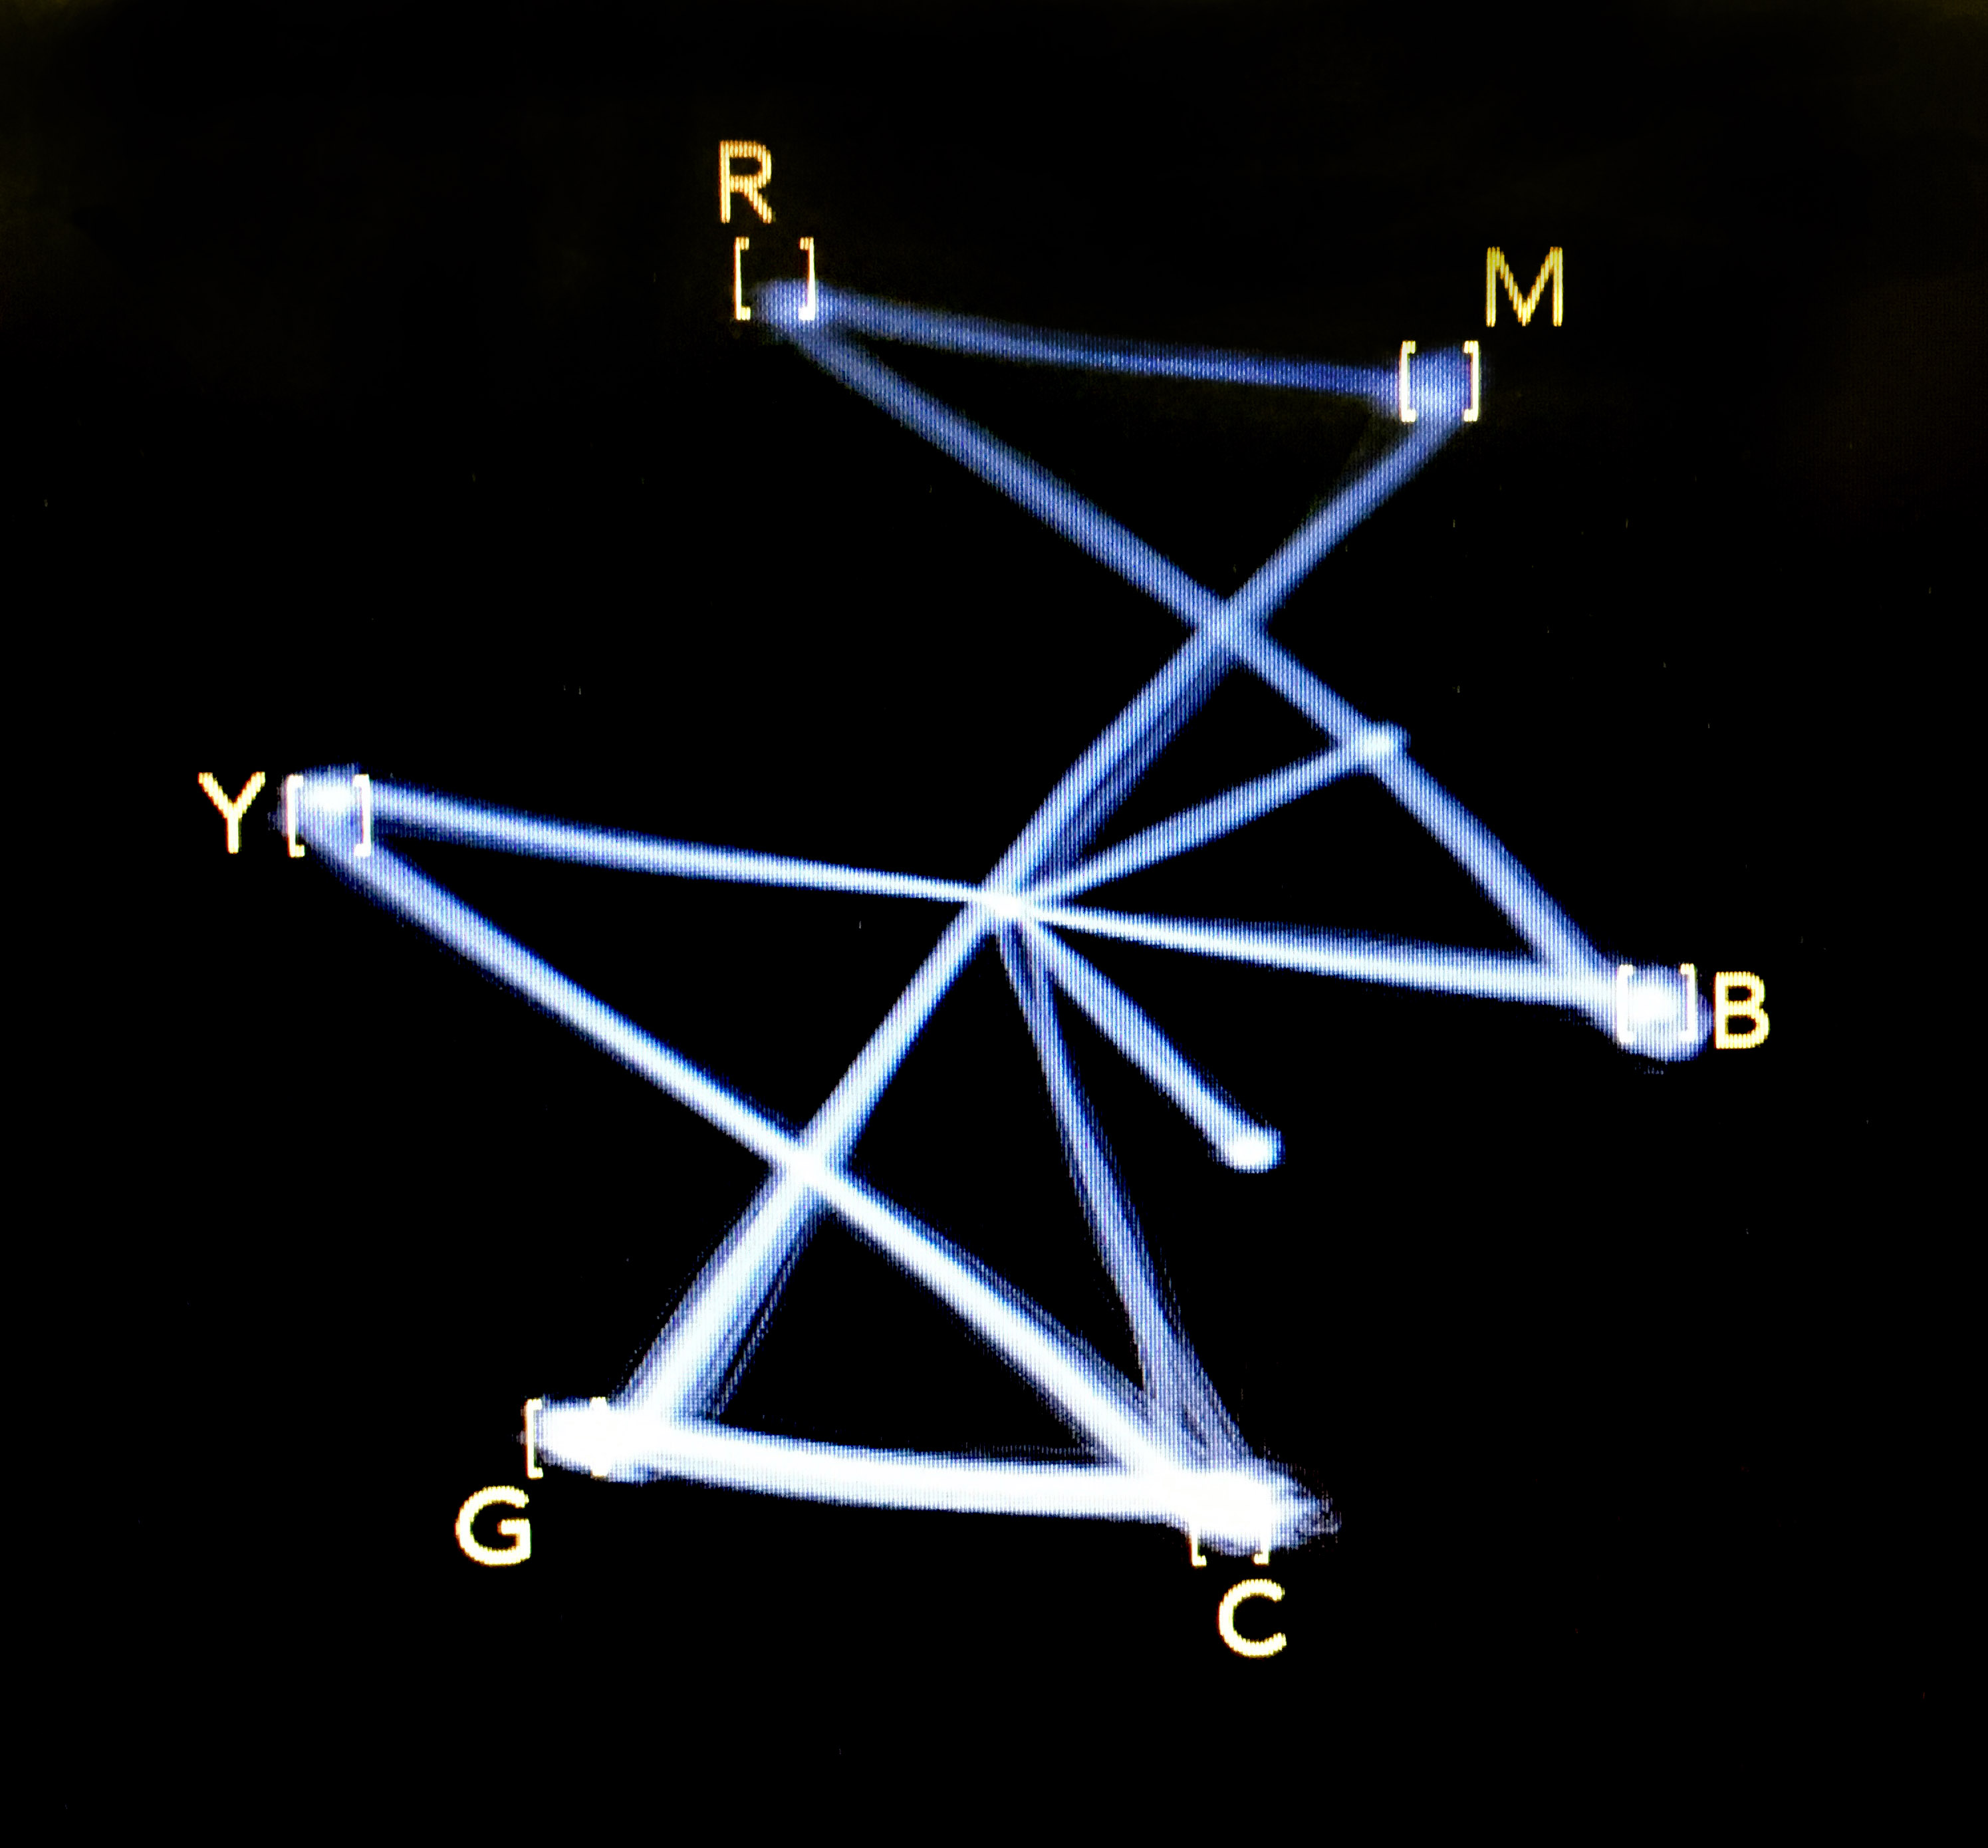
\includegraphics{images/vectorscope.jpg}
\caption{\label{fig:unnamed-chunk-1}Barres de calibration couleur sur vectorscope \citep{marsh_ColorBarsVectorscope_2016}}
\end{figure}

\hypertarget{sources}{%
\section{Sources}\label{sources}}

\begin{itemize}
\tightlist
\item
  \emph{GIT}\citep{torvalds_Git_2006} hébergé \href{https://github.com/tim-montmorency/543-traitement-video}{github.com/tim-montmorency/543-traitement-video}
\item
  \emph{Libre}\citep{stallman_GnuOrg_1983}
\item
  Écrit en \emph{RMarkdown}\citep{allaire_RmarkdownDynamicDocuments_2020}\\
\item
  Compilation via Bookdown\citep{xie_BookdownAuthoringBooks_2020}

  \begin{itemize}
  \tightlist
  \item
    \href{https://tim-montmorency.com/543-traitement-video/}{HTML}
  \item
    \href{https://tim-montmorency.com/543-traitement-video/traitement-video.pdf}{PDF}
  \item
    \href{https://tim-montmorency.com/543-traitement-video/traitement-video.epub}{EPUB}
  \end{itemize}
\item
  \href{https://github.com/tim-montmorency/543-traitement-video/blob/master/582543-traitement-video.bib}{Bibliographie Bibtex}
\end{itemize}

\hypertarget{mo-traitement-viduxe9o}{%
\chapter{582-543-MO Traitement vidéo}\label{mo-traitement-viduxe9o}}

\hypertarget{description-du-cours}{%
\section{Description du cours}\label{description-du-cours}}

\begin{itemize}
\tightlist
\item
  Techniques D'INTÉGRATION MULTIMÉDIA
\item
  Département des techniques d'intégration multimédia
\item
  582.A1
\item
  Pondération : 1-2-2
\item
  Unités: 1,66
\item
  Heures-contact : 45
\item
  Session : 4
\end{itemize}

Ce cours permet à l'étudiante ou l'étudiant d'enregistrer, de modifier et de traiter des images en temps réel.
L'étudiant sera appelé à appliquer des effets visuels aux images vidéo et à adapter les images en fonction de l'intégration.

\hypertarget{objectifs}{%
\section{Objectifs}\label{objectifs}}

\hypertarget{intuxe9grateur-et-ministuxe9riel}{%
\subsection{Intégrateur et ministériel}\label{intuxe9grateur-et-ministuxe9riel}}

\begin{itemize}
\tightlist
\item
  015J Traiter les images en mouvement
\end{itemize}

\hypertarget{apprentissages}{%
\subsection{Apprentissages}\label{apprentissages}}

\begin{itemize}
\tightlist
\item
  Adapter l'image en mouvement (Importance relative\,: 40\% )
\item
  Programmer des effets visuels interactifs (Importance relative\,: 40\% )
\item
  Intégrer l'image en mouvement interactive à une production médiatique (Importance relative\,: 20\% )
\end{itemize}

\hypertarget{pruxe9alables}{%
\section{Préalables}\label{pruxe9alables}}

\hypertarget{pruxe9alable-absolu-au-pruxe9sent-cours}{%
\subsection{Préalable absolu au présent cours~:}\label{pruxe9alable-absolu-au-pruxe9sent-cours}}

\begin{itemize}
\tightlist
\item
  582 413 MO Montage vidéo
\end{itemize}

\hypertarget{pruxe9alable-absolu-aux-cours-suivants}{%
\subsection{Préalable absolu aux cours suivants~:}\label{pruxe9alable-absolu-aux-cours-suivants}}

\begin{itemize}
\tightlist
\item
  582~513 MO Conception de projet multimédia
\item
  582 66B MO Expérience multimédia interactive
\item
  582 66G MO Production Web en entreprise
\end{itemize}

\hypertarget{muxe9thodologie}{%
\section{Méthodologie~}\label{muxe9thodologie}}

L'approche pédagogique de ce cours emprunte à celle employée dans les séminaires de recherche-création en média numérique. Une attention particulière est attribuée au partage de l'expérimentation en lien avec le sujet du cours. Différentes activités pédagogiques seront à l'honneur, notamment :

\begin{itemize}
\tightlist
\item
  Exposés magistraux
\item
  Démonstrations
\item
  Séances de questions
\item
  Présentations étudiantes
\item
  Valorisation des apprentissages autonomes
\item
  Utilisation créative de logiciels
\item
  Travaux pratiques itératifs
\end{itemize}

\hypertarget{duxe9veloppement}{%
\section{Développement}\label{duxe9veloppement}}

\hypertarget{attitudes-professionnelles}{%
\subsection{Attitudes professionnelles}\label{attitudes-professionnelles}}

\begin{itemize}
\tightlist
\item
  Curiosité
\item
  Capacité de partage
\item
  Créativité
\item
  Esprit critique
\item
  Sens esthétique
\end{itemize}

\hypertarget{habiletuxe9s-transdisciplinaires}{%
\subsection{Habiletés transdisciplinaires}\label{habiletuxe9s-transdisciplinaires}}

\begin{itemize}
\tightlist
\item
  Profil \textbf{technologies de l'information et de la communication (TIC)}
\item
  Les étudiantes et étudiants auront à exploiter les TIC de manière efficace et responsable.
\item
  Recherche, traitement et présentation de l'information.
\end{itemize}

\hypertarget{contexte-particulier-dapprentissage}{%
\section{Contexte particulier d'apprentissage}\label{contexte-particulier-dapprentissage}}

\begin{itemize}
\tightlist
\item
  À distance; synchrone.
\item
  Possibilité d'utiliser le laboratoire informatique et le studio si nécessaire.
\end{itemize}

\hypertarget{fiche-technique}{%
\subsection{Fiche technique}\label{fiche-technique}}

\begin{itemize}
\tightlist
\item
  Ordinateurs, projecteurs à haute luminosité ou télévision, haut-parleurs professionnels, casque audio, matériel disponible pour TIM
\item
  Logiciels de montage vidéo et traitemet vidéo en temps réel
\item
  Languages et protocoles de paramétrage\\
\item
  Technicienne ou technicien en travaux pratiques
\end{itemize}

\hypertarget{contenus_essentiels}{%
\section{Contenus essentiels}\label{contenus_essentiels}}

\hypertarget{survol-historique}{%
\subsection{Survol historique}\label{survol-historique}}

\begin{itemize}
\tightlist
\item
  \protect\hyperlink{evolution_historique}{Évolution historique du traitement vidéo dans les différentes formes d'art}

  \begin{itemize}
  \tightlist
  \item
    \protect\hyperlink{evolution_historique_performance}{Performance}
  \item
    \protect\hyperlink{evolution_historique_installation}{Installation}
  \item
    \protect\hyperlink{evolution_historique_technologies}{Évolution des technologies associées}
  \end{itemize}
\item
  \protect\hyperlink{evolution_historique_language}{Langages et moyens expressifs de l'image en mouvement}
\end{itemize}

\hypertarget{fondements-techniques}{%
\subsection{Fondements techniques}\label{fondements-techniques}}

\begin{itemize}
\tightlist
\item
  \protect\hyperlink{lexique_fichiers}{Formats de fichiers}
\item
  \protect\hyperlink{lexique_encodage}{Encodage des vidéos}\\
\item
  \protect\hyperlink{aquerir_captation}{Captation vidéo en temps réel}
\item
  \protect\hyperlink{traiter_logiciels}{Logiciels de traitement vidéo en temps réel et d'interactivité}
\item
  \protect\hyperlink{programmer_logiciels}{Logiciels de programmation nodale}
\item
  Notions de traitement vidéo

  \begin{itemize}
  \tightlist
  \item
    pixels
  \item
    couleurs
  \item
    texture
  \item
    matrice
  \item
    mémoire tampon
  \item
    alpha channel
  \item
    rendu OpenGL
  \end{itemize}
\end{itemize}

\hypertarget{traitement-de-limage-en-mouvement}{%
\subsection{Traitement de l'image en mouvement}\label{traitement-de-limage-en-mouvement}}

\begin{itemize}
\tightlist
\item
  Usage de capture vidéo en temps réel\\
\item
  Effets visuels et filtres applicables en temps réel sur des matériaux visuels\\
\item
  Traitement visuel en temps réel à l'aide d'effets et de logiciels de programmation multimédia et nodale
\item
  Flot de données entre les objets du logiciel
\item
  Exploitation des fonctions des logiciels de traitement vidéo en temps réel
\item
  Utilisation de nuanceurs (shaders)
\end{itemize}

\hypertarget{programmation-deffets-visuels}{%
\subsection{Programmation d'effets visuels}\label{programmation-deffets-visuels}}

\begin{itemize}
\tightlist
\item
  Programmation de compositions visuelles génératives
\item
  Réalisation d'un échantillonneur/mélangeur visuel
\item
  Programmation pour contrôler la lecture vidéo,

  \begin{itemize}
  \tightlist
  \item
    montage temps réel
  \item
    niveau des couleurs
  \item
    alpha channel\\
  \end{itemize}
\item
  Programmation nodale pour créer des effets en temps réel

  \begin{itemize}
  \tightlist
  \item
    position
  \item
    rotation
  \item
    dimensions
  \item
    mixage d'images
  \item
    incrustation
  \item
    distorsion
  \item
    délais
  \item
    rétroaction (feedback)
  \item
    modification de couleurs
  \item
    chromakey
  \item
    lumière
  \item
    fumée
  \item
    texture
  \end{itemize}
\item
  Nuanceurs (shaders)\,: vertex, pixel et géométrie
\end{itemize}

\hypertarget{image-en-mouvement-et-interactivituxe9}{%
\subsection{Image en mouvement et interactivité}\label{image-en-mouvement-et-interactivituxe9}}

\begin{itemize}
\tightlist
\item
  Intégration des composantes dans une production interactive
\item
  Configuration logicielle et matérielle d'une production interactive\\
\item
  Conceptualisation et scénarisation d'un projet visuel interactif\\
\item
  Captation de mouvement et de présence
\item
  Programmation de la captation de mouvement et de présence
\item
  Utilisation d'interfaces de contrôle interactives
\item
  Utilisation d'OSC, MIDI, DMX ou ArtNet pour interagir avec d'autres logiciels et interfaces de contrôle
\end{itemize}

\hypertarget{gestion-de-projets}{%
\subsection{Gestion de projets}\label{gestion-de-projets}}

\begin{itemize}
\tightlist
\item
  Schématisation
\item
  Prototypage
\item
  Gestion de banques d'images
\item
  Optimisation des performances de l'application
\item
  Test de contrôle de qualité
\item
  Préréglages
\item
  Optimisation de la programmation et commentaires
\item
  Console de débogage
\item
  Exportation de projets
\item
  Formats de sauvegarde\\
\item
  Application autonome
\item
  Sauvegarde et archivage des médias
\item
  Ajustement des effets visuels en fonction des tests
\end{itemize}

\hypertarget{calendrier}{%
\chapter{Calendrier}\label{calendrier}}

\href{https://www.cmontmorency.qc.ca/wp-content/uploads/images/college/administration/CALENDRIER-SCOLAIRE-2020-2021.pdf}{Calendrier Collège Montmorency 2020-2021}

\begin{table}

\caption{\label{tab:calendrier}Calendrier}
\centering
\begin{tabular}[t]{>{\raggedright\arraybackslash}p{.5em}>{\raggedright\arraybackslash}p{10em}>{\raggedright\arraybackslash}p{10em}}
\toprule
Séance & OBJECTIFS ABORDÉS EN CLASSE & ACTIVITÉS AUTONOMES\\
\midrule
[1; 3 février](\#semaine\_1) & Plan de cour; Survol [corpus artistique](\#corpus); Consignes [Présentation corpus vidéo](\#sommatif\_1); & Recherche d'un sujet [Présentation corpus vidéo](\#sommatif\_1)\\
[2; 10 février](\#semaine\_2) & [Historique du traitement vidéo](\#evolution\_historique); Formatif Préapprobation [Présentation corpus Vidéo](\#sommatif\_1) & Préparation [Présentation corpus vidéo](\#sommatif\_1)\\
[3; 17 février](\#semaine\_3) & Sommatif [Présentation corpus Vidéo](\#sommatif\_1) & \\
[4; 24 février](\#semaine\_4) & [Composantes du signal vidéo](\#lexique); [Acquérir l'image en mouvement](\#acquerir); [Échantillonner l'image en mouvement](\#echantillonner); Consignes [Question traitement vidéo](\#sommatif\_2) & Préparation [Question traitement vidéo](\#sommatif\_2)\\
[X; 3 mars](\#semaine\_5) & Journées de rattrapage (Pas de cours) & \\
\addlinespace
[5; 10 mars](\#semaine\_6) & [Traiter l'image en mouvement](\#traiter); Formatif Préapprobation [Question traitement vidéo](\#sommatif\_2) & Soumettre [Question traitement vidéo](\#sommatif\_2)\\
[6; 17 mars](\#semaine\_7) & Consignes [Palette vidéo interactive](\#sommatif\_4); Sommatif [Quiz traitement vidéo](\#sommatif\_3) & Préparation [Palette vidéo interactive](\#sommatif\_4)\\
[7; 24 mars](\#semaine\_8) & [Programmer des sources visuelles](\#programmer) & Préparation [Palette vidéo interactive](\#sommatif\_4)\\
[8; 31 mars](\#semaine\_9) & [Interagir avec des sources vidéo](\#interagir) & Préparation [Palette vidéo interactive](\#sommatif\_4)\\
[X; 7 avril](\#semaine\_10) & Congé (Pas de cours) & \\
\addlinespace
[9; 14 avril](\#semaine\_11) & Suite [Programmer des sources visuelles](\#programmer) et [Interagir avec des sources vidéo](\#interagir) & Préparation [Palette vidéo interactive](\#sommatif\_4)\\
[10; 21 avril](\#semaine\_12) & Sommatif [Palette vidéo interactive](\#sommatif\_4) & \\
[11; 28 avril](\#semaine\_13) & [Déployer un projet vidéo temps réel](\#deployer); Consignes [performance audiovisuelle temps réel](\#sommatif\_5) & Préparation [performance audiovisuelle temps réel](\#sommatif\_5)\\
[12; 5 mai](\#semaine\_14) & Suite [Déployer un projet vidéo temps réel](\#deployer) & Préparation [performance audiovisuelle temps réel](\#sommatif\_5)\\
[13; 12 mai](\#semaine\_15) & Préparation [performance audiovisuelle temps réel](\#sommatif\_5) & Préparation [performance audiovisuelle temps réel](\#sommatif\_5)\\
\addlinespace
[14; 18 mai ](\#semaine\_16) & Exceptionnellement un mardi, [performance audiovisuelle temps réel](\#sommatif\_5); & Rédaction du document accompagnateur [performance audiovisuelle temps réel ](\#sommatif\_5)\\
[X; 19 mai](\#semaine\_17) & Épreuve uniforme de français (Pas de cours) & Rédaction document [performance audiovisuelle temps réel ](\#sommatif\_5)\\
[15; 25 mai](\#semaine\_18) & Remise du document accompagnateur [performance audiovisuelle temps réel ](\#sommatif\_5) & \\
\bottomrule
\end{tabular}
\end{table}

\hypertarget{semaine_1}{%
\section{\texorpdfstring{Séance \protect\hyperlink{semaine_1}{1; 3 février}}{Séance 1; 3 février}}\label{semaine_1}}

\hypertarget{objectifs-aborduxe9s-en-classe}{%
\subsection{OBJECTIFS ABORDÉS EN CLASSE}\label{objectifs-aborduxe9s-en-classe}}

Plan de cour Survol \protect\hyperlink{corpus}{corpus artistique} Consignes \protect\hyperlink{sommatif_1}{Présentation corpus vidéo}

\hypertarget{activituxe9s-autonomes}{%
\subsection{ACTIVITÉS AUTONOMES}\label{activituxe9s-autonomes}}

Recherche d'un sujet \protect\hyperlink{sommatif_1}{Présentation corpus vidéo}

\hypertarget{semaine_2}{%
\section{\texorpdfstring{Séance \protect\hyperlink{semaine_2}{2; 10 février}}{Séance 2; 10 février}}\label{semaine_2}}

\hypertarget{objectifs-aborduxe9s-en-classe-1}{%
\subsection{OBJECTIFS ABORDÉS EN CLASSE}\label{objectifs-aborduxe9s-en-classe-1}}

\protect\hyperlink{evolution_historique}{Historique du traitement vidéo} Formatif Préapprobation \protect\hyperlink{sommatif_1}{Présentation corpus Vidéo}

\hypertarget{activituxe9s-autonomes-1}{%
\subsection{ACTIVITÉS AUTONOMES}\label{activituxe9s-autonomes-1}}

Préparation \protect\hyperlink{sommatif_1}{Présentation corpus vidéo}

\hypertarget{semaine_3}{%
\section{\texorpdfstring{Séance \protect\hyperlink{semaine_3}{3; 17 février}}{Séance 3; 17 février}}\label{semaine_3}}

\hypertarget{objectifs-aborduxe9s-en-classe-2}{%
\subsection{OBJECTIFS ABORDÉS EN CLASSE}\label{objectifs-aborduxe9s-en-classe-2}}

Sommatif \protect\hyperlink{sommatif_1}{Présentation corpus Vidéo}

\hypertarget{activituxe9s-autonomes-2}{%
\subsection{ACTIVITÉS AUTONOMES}\label{activituxe9s-autonomes-2}}

\hypertarget{semaine_4}{%
\section{\texorpdfstring{Séance \protect\hyperlink{semaine_4}{4; 24 février}}{Séance 4; 24 février}}\label{semaine_4}}

\hypertarget{objectifs-aborduxe9s-en-classe-3}{%
\subsection{OBJECTIFS ABORDÉS EN CLASSE}\label{objectifs-aborduxe9s-en-classe-3}}

\protect\hyperlink{lexique}{Composantes du signal vidéo} \protect\hyperlink{acquerir}{Acquérir l'image en mouvement} \protect\hyperlink{echantillonner}{Échantillonner l'image en mouvement} Consignes \protect\hyperlink{sommatif_2}{Question traitement vidéo}

\hypertarget{activituxe9s-autonomes-3}{%
\subsection{ACTIVITÉS AUTONOMES}\label{activituxe9s-autonomes-3}}

Préparation \protect\hyperlink{sommatif_2}{Question traitement vidéo}

\hypertarget{semaine_5}{%
\section{\texorpdfstring{Séance \protect\hyperlink{semaine_5}{X; 3 mars}}{Séance X; 3 mars}}\label{semaine_5}}

\hypertarget{objectifs-aborduxe9s-en-classe-4}{%
\subsection{OBJECTIFS ABORDÉS EN CLASSE}\label{objectifs-aborduxe9s-en-classe-4}}

Journées de rattrapage (Pas de cours)

\hypertarget{activituxe9s-autonomes-4}{%
\subsection{ACTIVITÉS AUTONOMES}\label{activituxe9s-autonomes-4}}

\hypertarget{semaine_6}{%
\section{\texorpdfstring{Séance \protect\hyperlink{semaine_6}{5; 10 mars}}{Séance 5; 10 mars}}\label{semaine_6}}

\hypertarget{objectifs-aborduxe9s-en-classe-5}{%
\subsection{OBJECTIFS ABORDÉS EN CLASSE}\label{objectifs-aborduxe9s-en-classe-5}}

\protect\hyperlink{traiter}{Traiter l'image en mouvement} Formatif Préapprobation \protect\hyperlink{sommatif_2}{Question traitement vidéo}

\hypertarget{activituxe9s-autonomes-5}{%
\subsection{ACTIVITÉS AUTONOMES}\label{activituxe9s-autonomes-5}}

Soumettre \protect\hyperlink{sommatif_2}{Question traitement vidéo}

\hypertarget{semaine_7}{%
\section{\texorpdfstring{Séance \protect\hyperlink{semaine_7}{6; 17 mars}}{Séance 6; 17 mars}}\label{semaine_7}}

\hypertarget{objectifs-aborduxe9s-en-classe-6}{%
\subsection{OBJECTIFS ABORDÉS EN CLASSE}\label{objectifs-aborduxe9s-en-classe-6}}

Consignes \protect\hyperlink{sommatif_4}{Palette vidéo interactive} Sommatif \protect\hyperlink{sommatif_3}{Quiz traitement vidéo}

\hypertarget{activituxe9s-autonomes-6}{%
\subsection{ACTIVITÉS AUTONOMES}\label{activituxe9s-autonomes-6}}

Préparation \protect\hyperlink{sommatif_4}{Palette vidéo interactive}

\hypertarget{semaine_8}{%
\section{\texorpdfstring{Séance \protect\hyperlink{semaine_8}{7; 24 mars}}{Séance 7; 24 mars}}\label{semaine_8}}

\hypertarget{objectifs-aborduxe9s-en-classe-7}{%
\subsection{OBJECTIFS ABORDÉS EN CLASSE}\label{objectifs-aborduxe9s-en-classe-7}}

\protect\hyperlink{programmer}{Programmer des sources visuelles}

\hypertarget{activituxe9s-autonomes-7}{%
\subsection{ACTIVITÉS AUTONOMES}\label{activituxe9s-autonomes-7}}

Préparation \protect\hyperlink{sommatif_4}{Palette vidéo interactive}

\hypertarget{semaine_9}{%
\section{\texorpdfstring{Séance \protect\hyperlink{semaine_9}{8; 31 mars}}{Séance 8; 31 mars}}\label{semaine_9}}

\hypertarget{objectifs-aborduxe9s-en-classe-8}{%
\subsection{OBJECTIFS ABORDÉS EN CLASSE}\label{objectifs-aborduxe9s-en-classe-8}}

\protect\hyperlink{interagir}{Interagir avec des sources vidéo}

\hypertarget{activituxe9s-autonomes-8}{%
\subsection{ACTIVITÉS AUTONOMES}\label{activituxe9s-autonomes-8}}

Préparation \protect\hyperlink{sommatif_4}{Palette vidéo interactive}

\hypertarget{semaine_10}{%
\section{\texorpdfstring{Séance \protect\hyperlink{semaine_10}{X; 7 avril}}{Séance X; 7 avril}}\label{semaine_10}}

\hypertarget{objectifs-aborduxe9s-en-classe-9}{%
\subsection{OBJECTIFS ABORDÉS EN CLASSE}\label{objectifs-aborduxe9s-en-classe-9}}

Congé (Pas de cours)

\hypertarget{activituxe9s-autonomes-9}{%
\subsection{ACTIVITÉS AUTONOMES}\label{activituxe9s-autonomes-9}}

\hypertarget{semaine_11}{%
\section{\texorpdfstring{Séance \protect\hyperlink{semaine_11}{9; 14 avril}}{Séance 9; 14 avril}}\label{semaine_11}}

\hypertarget{objectifs-aborduxe9s-en-classe-10}{%
\subsection{OBJECTIFS ABORDÉS EN CLASSE}\label{objectifs-aborduxe9s-en-classe-10}}

Suite \protect\hyperlink{programmer}{Programmer des sources visuelles} et \protect\hyperlink{interagir}{Interagir avec des sources vidéo}

\hypertarget{activituxe9s-autonomes-10}{%
\subsection{ACTIVITÉS AUTONOMES}\label{activituxe9s-autonomes-10}}

Préparation \protect\hyperlink{sommatif_4}{Palette vidéo interactive}

\hypertarget{semaine_12}{%
\section{\texorpdfstring{Séance \protect\hyperlink{semaine_12}{10; 21 avril}}{Séance 10; 21 avril}}\label{semaine_12}}

\hypertarget{objectifs-aborduxe9s-en-classe-11}{%
\subsection{OBJECTIFS ABORDÉS EN CLASSE}\label{objectifs-aborduxe9s-en-classe-11}}

Sommatif \protect\hyperlink{sommatif_4}{Palette vidéo interactive}

\hypertarget{activituxe9s-autonomes-11}{%
\subsection{ACTIVITÉS AUTONOMES}\label{activituxe9s-autonomes-11}}

\hypertarget{semaine_13}{%
\section{\texorpdfstring{Séance \protect\hyperlink{semaine_13}{11; 28 avril}}{Séance 11; 28 avril}}\label{semaine_13}}

\hypertarget{objectifs-aborduxe9s-en-classe-12}{%
\subsection{OBJECTIFS ABORDÉS EN CLASSE}\label{objectifs-aborduxe9s-en-classe-12}}

\protect\hyperlink{deployer}{Déployer un projet vidéo temps réel} Consignes \protect\hyperlink{sommatif_5}{performance audiovisuelle temps réel}

\hypertarget{activituxe9s-autonomes-12}{%
\subsection{ACTIVITÉS AUTONOMES}\label{activituxe9s-autonomes-12}}

Préparation \protect\hyperlink{sommatif_5}{performance audiovisuelle temps réel}

\hypertarget{semaine_14}{%
\section{\texorpdfstring{Séance \protect\hyperlink{semaine_14}{12; 5 mai}}{Séance 12; 5 mai}}\label{semaine_14}}

\hypertarget{objectifs-aborduxe9s-en-classe-13}{%
\subsection{OBJECTIFS ABORDÉS EN CLASSE}\label{objectifs-aborduxe9s-en-classe-13}}

Suite \protect\hyperlink{deployer}{Déployer un projet vidéo temps réel}

\hypertarget{activituxe9s-autonomes-13}{%
\subsection{ACTIVITÉS AUTONOMES}\label{activituxe9s-autonomes-13}}

Préparation \protect\hyperlink{sommatif_5}{performance audiovisuelle temps réel}

\hypertarget{semaine_15}{%
\section{\texorpdfstring{Séance \protect\hyperlink{semaine_15}{13; 12 mai}}{Séance 13; 12 mai}}\label{semaine_15}}

\hypertarget{objectifs-aborduxe9s-en-classe-14}{%
\subsection{OBJECTIFS ABORDÉS EN CLASSE}\label{objectifs-aborduxe9s-en-classe-14}}

Préparation \protect\hyperlink{sommatif_5}{performance audiovisuelle temps réel}

\hypertarget{activituxe9s-autonomes-14}{%
\subsection{ACTIVITÉS AUTONOMES}\label{activituxe9s-autonomes-14}}

Préparation \protect\hyperlink{sommatif_5}{performance audiovisuelle temps réel}

\hypertarget{semaine_16}{%
\section{\texorpdfstring{Séance \protect\hyperlink{semaine_16}{14; 18 mai}}{Séance 14; 18 mai}}\label{semaine_16}}

\hypertarget{objectifs-aborduxe9s-en-classe-15}{%
\subsection{OBJECTIFS ABORDÉS EN CLASSE}\label{objectifs-aborduxe9s-en-classe-15}}

Exceptionnellement un mardi, \protect\hyperlink{sommatif_5}{performance audiovisuelle temps réel}

\hypertarget{activituxe9s-autonomes-15}{%
\subsection{ACTIVITÉS AUTONOMES}\label{activituxe9s-autonomes-15}}

Rédaction du document accompagnateur \protect\hyperlink{sommatif_5}{performance audiovisuelle temps réel}

\hypertarget{semaine_17}{%
\section{\texorpdfstring{Séance \protect\hyperlink{semaine_17}{X; 19 mai}}{Séance X; 19 mai}}\label{semaine_17}}

\hypertarget{objectifs-aborduxe9s-en-classe-16}{%
\subsection{OBJECTIFS ABORDÉS EN CLASSE}\label{objectifs-aborduxe9s-en-classe-16}}

Épreuve uniforme de français (Pas de cours)

\hypertarget{activituxe9s-autonomes-16}{%
\subsection{ACTIVITÉS AUTONOMES}\label{activituxe9s-autonomes-16}}

Rédaction document \protect\hyperlink{sommatif_5}{performance audiovisuelle temps réel}

\hypertarget{semaine_18}{%
\section{\texorpdfstring{Séance \protect\hyperlink{semaine_18}{15; 25 mai}}{Séance 15; 25 mai}}\label{semaine_18}}

\hypertarget{objectifs-aborduxe9s-en-classe-17}{%
\subsection{OBJECTIFS ABORDÉS EN CLASSE}\label{objectifs-aborduxe9s-en-classe-17}}

Remise du document accompagnateur \protect\hyperlink{sommatif_5}{performance audiovisuelle temps réel}

\hypertarget{activituxe9s-autonomes-17}{%
\subsection{ACTIVITÉS AUTONOMES}\label{activituxe9s-autonomes-17}}

\hypertarget{exercices}{%
\chapter{Exercices}\label{exercices}}

\hypertarget{sommatif_1}{%
\section{Présentation corpus vidéo}\label{sommatif_1}}

\begin{itemize}
\tightlist
\item
  Présentation de type partage d'écran de \textasciitilde5 minutes
\item
  Sommatif (15\%)
\item
  Individuel
\end{itemize}

\hypertarget{consignes}{%
\subsection{Consignes}\label{consignes}}

\begin{itemize}
\tightlist
\item
  Choisir et présenter un court extrait médiatique comprenant un procédé de traitement vidéo original

  \begin{itemize}
  \tightlist
  \item
    Se référer à la section \protect\hyperlink{corpus}{corpus} pour une liste d'artistes potentiellement inspirants
  \end{itemize}
\item
  Traiter synthétiquement son contexte artistique et historique

  \begin{itemize}
  \tightlist
  \item
    Auteur

    \begin{itemize}
    \tightlist
    \item
      Nom, année de naissance (si disponible), nationalité (ville, pays (si disponible)),

      \begin{itemize}
      \tightlist
      \item
        ex: Marina Abramovic, 1946 à Belgrade, Yougoslavie (aujourd'hui Serbie-Monténégro)
      \end{itemize}
    \end{itemize}
  \item
    Contexte de diffusion de l'oeuvre

    \begin{itemize}
    \tightlist
    \item
      Titre

      \begin{itemize}
      \tightlist
      \item
        ex. Twenty four hour Psycho
      \end{itemize}
    \item
      médium, durée, date de parution

      \begin{itemize}
      \tightlist
      \item
        ex. Installation vidéo à 6 canaux, couleur, son, 12 minutes, 1997
      \end{itemize}
    \end{itemize}
  \end{itemize}
\item
  Décrire une technique de traitement vidéo employée

  \begin{itemize}
  \tightlist
  \item
    Ex. La chronophotographie (décrire la technique) fut employé pour (décrire une motivation artistique)
  \end{itemize}
\item
  Présenter une hypothèse à la question suivante :

  \begin{itemize}
  \tightlist
  \item
    Est-ce que ce procédé de traitement vidéo étudié pourrait être produit en temps réel?

    \begin{itemize}
    \tightlist
    \item
      si oui, comment?
    \item
      sinon, pourquoi?
    \end{itemize}
  \end{itemize}
\end{itemize}

\hypertarget{sommatif_2}{%
\section{Rédaction d'une question portant sur le traitement vidéo}\label{sommatif_2}}

\begin{itemize}
\tightlist
\item
  Rédaction dans un tableur Excel en ligne d'une question, une bonne réponse et 3 réponses erronées\\
\item
  Sommatif (10\%)
\item
  Individuel
\end{itemize}

\hypertarget{consignes-1}{%
\subsection{Consignes}\label{consignes-1}}

\begin{itemize}
\tightlist
\item
  Rédiger une question pertinente et originale sur le traitement vidéo
\item
  Inscrire une réponse adéquate
\item
  Inventer trois réponses erronées (formatif)
\item
  Se référer aux \href{}{contenus essentiels}
\end{itemize}

\hypertarget{sommatif_3}{%
\section{Jeu-questionnaire théorique}\label{sommatif_3}}

\begin{itemize}
\tightlist
\item
  Formulaire en ligne à répondre avant la date prévue
\item
  Sommatif (15\%)
\item
  Individuel
\end{itemize}

\hypertarget{consignes-2}{%
\subsection{Consignes}\label{consignes-2}}

\begin{itemize}
\tightlist
\item
  Répondre aux questions dans le formulaire avant l'échéance
\end{itemize}

\hypertarget{sommatif_4}{%
\section{Palette de scènes vidéo interactives}\label{sommatif_4}}

\begin{itemize}
\tightlist
\item
  Présentation de type partage d'écran \textasciitilde5 minutes
\item
  Sommatif 25\%
\item
  individuel
\end{itemize}

\hypertarget{consignes-3}{%
\subsection{Consignes}\label{consignes-3}}

\begin{itemize}
\tightlist
\item
  Assembler une palette de 8 scènes vidéo comprenant

  \begin{itemize}
  \tightlist
  \item
    échantillons vidéo
  \item
    caméra vidéo
  \item
    source HTML
  \item
    source nuancier
  \item
    etc.
  \end{itemize}
\item
  Démontrer

  \begin{itemize}
  \tightlist
  \item
    Capacité d'adapter l'image en mouvement
  \item
    Capacité d'interagir avec des effets visuels interactifs
  \item
    Maitrise technique
  \item
    Créativité
  \end{itemize}
\end{itemize}

\hypertarget{sommatif_5}{%
\section{Performance audiovisuelle temps réel et document accompagnateur}\label{sommatif_5}}

\begin{itemize}
\tightlist
\item
  35\% individuel, produit en équipe
\item
  Présentation courte au sein d'une diffusion audiovisuelle continue (Stream)
\item
  Présenté lors de la ruche u
\item
  Signal issu d'un processus de mélange de signaux en temps réel
\item
  Variation en temps réel de paramètres vidéo programmés
\end{itemize}

\hypertarget{consignes-4}{%
\subsection{Consignes}\label{consignes-4}}

\hypertarget{performance-audiovisuelle-temps-ruxe9el}{%
\subsubsection{Performance audiovisuelle temps réel}\label{performance-audiovisuelle-temps-ruxe9el}}

\begin{itemize}
\tightlist
\item
  Activité concertée avec le cours de Conception sonore interactive
\item
  le traitement vidéo doit être effectué en temps réel
\item
  Présentation de type streaming lors de la ruche (mardi)
\item
  Tous les groupes doivent diffuser ce jour-là
\end{itemize}

\hypertarget{consignes-document-accompagnateur}{%
\subsubsection{Consignes (document accompagnateur}\label{consignes-document-accompagnateur}}

\begin{itemize}
\tightlist
\item
  Remise avant le 26 mai d'un texte individuel expliquant dans un langage approprié et précis les éléments suivant:

  \begin{itemize}
  \tightlist
  \item
    L'implication au sein du projet
  \item
    Les intentions artistiques
  \item
    Les défis techniques
  \item
    La démarche
  \item
    L'inspiration
  \item
    Le fonctionnement technique du travail
  \item
    Ce qui aurait pu améliorer le résultat
  \end{itemize}
\item
  N.B. : un document par étudiant, soumis à la fois au cours de Traitement vidéo ainsi qu'au cours de Conception sonore interactive. Seuls les éléments décrits dans ce texte compteront à l'évaluation. Ne pas oublier de détailler autant l'aspect visuel que le sonore.
\end{itemize}

\hypertarget{corpus}{%
\chapter{Corpus chronologique d'artistes}\label{corpus}}

(non exaustif bien sur)

\hypertarget{les-origines-de-lart-viduxe9o}{%
\section{Les origines de l'art vidéo}\label{les-origines-de-lart-viduxe9o}}

\hypertarget{edward-muybridge}{%
\subsection{Edward Muybridge}\label{edward-muybridge}}

\begin{itemize}
\tightlist
\item
  \url{http://www.artwiki.fr/?EdwardMuybridge}
\end{itemize}

\hypertarget{georges-muxe9lies}{%
\subsection{Georges Mélies}\label{georges-muxe9lies}}

\begin{itemize}
\tightlist
\item
  \url{http://www.artwiki.fr/?GeorgesMelies}
\end{itemize}

\hypertarget{etienne-jules-marey}{%
\subsection{Etienne-Jules Marey}\label{etienne-jules-marey}}

\begin{itemize}
\tightlist
\item
  \url{http://www.artwiki.fr/?EtiennejulesMarey}
\end{itemize}

\hypertarget{dziga-vertov}{%
\subsection{Dziga Vertov}\label{dziga-vertov}}

\begin{itemize}
\tightlist
\item
  \url{http://www.artwiki.fr/?DzigaVertov}
\end{itemize}

\hypertarget{futurisme-et-lart-viduxe9o}{%
\subsection{Futurisme et l'art vidéo}\label{futurisme-et-lart-viduxe9o}}

\begin{itemize}
\tightlist
\item
  \url{http://www.artwiki.fr/?FuturismeArtvideo}
\end{itemize}

\hypertarget{marcel-duchamp}{%
\subsection{Marcel Duchamp}\label{marcel-duchamp}}

\begin{itemize}
\tightlist
\item
  \url{http://www.artwiki.fr/?MarcelduchampEcologie}
\end{itemize}

\hypertarget{les-balbutiements}{%
\section{Les balbutiements}\label{les-balbutiements}}

\hypertarget{stan-brakhage}{%
\subsection{Stan Brakhage}\label{stan-brakhage}}

\begin{itemize}
\tightlist
\item
  \url{http://www.artwiki.fr/?StanBrakhage}
\end{itemize}

\hypertarget{john-milton-cage}{%
\subsection{John Milton Cage}\label{john-milton-cage}}

\begin{itemize}
\tightlist
\item
  \url{http://www.artwiki.fr/?JohnCage}
\end{itemize}

\hypertarget{fluxus}{%
\subsection{Fluxus}\label{fluxus}}

\begin{itemize}
\tightlist
\item
  \url{http://www.artwiki.fr/?LartvideoFluxus}
\end{itemize}

\hypertarget{norman-mclaren}{%
\subsection{Norman McLaren}\label{norman-mclaren}}

\begin{itemize}
\tightlist
\item
  \url{http://www.artwiki.fr/?NormanMcLaren}
\end{itemize}

\hypertarget{section}{%
\section{1960}\label{section}}

\hypertarget{nam-june-paik}{%
\subsection{Nam June Paik}\label{nam-june-paik}}

\begin{itemize}
\tightlist
\item
  \url{http://www.artwiki.fr/?NamjunePaik}
\item
  \url{https://fr.wikipedia.org/wiki/Nam_June_Paik}
\end{itemize}

\hypertarget{wolf-vostell}{%
\subsection{Wolf Vostell}\label{wolf-vostell}}

\begin{itemize}
\tightlist
\item
  \url{http://www.artwiki.fr/?WolfVostell}
\end{itemize}

\hypertarget{les-levine}{%
\subsection{Les Levine}\label{les-levine}}

\begin{itemize}
\tightlist
\item
  \url{http://www.artwiki.fr/?LesLevine}
\end{itemize}

\hypertarget{section-1}{%
\section{1970}\label{section-1}}

\hypertarget{valie-export}{%
\subsection{Valie Export}\label{valie-export}}

\begin{itemize}
\tightlist
\item
  \url{http://www.artwiki.fr/?ValieExport}
\end{itemize}

\hypertarget{frank-gillette}{%
\subsection{Frank Gillette}\label{frank-gillette}}

\begin{itemize}
\tightlist
\item
  \url{http://www.artwiki.fr/?FrankGillette}
\end{itemize}

\hypertarget{michael-snow}{%
\subsection{Michael Snow}\label{michael-snow}}

\begin{itemize}
\tightlist
\item
  \url{http://www.artwiki.fr/?MichaelSnow}
\end{itemize}

\hypertarget{jud-yalkut}{%
\subsection{Jud Yalkut}\label{jud-yalkut}}

\begin{itemize}
\tightlist
\item
  \url{http://www.artwiki.fr/?JudYalkut}
\end{itemize}

\hypertarget{shigeko-kubota}{%
\subsection{Shigeko Kubota}\label{shigeko-kubota}}

\begin{itemize}
\tightlist
\item
  \url{http://www.artwiki.fr/?ShigekoKubota}
\end{itemize}

\hypertarget{marina-abramovic-ulay}{%
\subsection{Marina Abramovic \& Ulay}\label{marina-abramovic-ulay}}

\begin{itemize}
\tightlist
\item
  \url{http://www.artwiki.fr/?AbramoviculayVideo70}
\end{itemize}

\hypertarget{contemporains}{%
\section{Contemporains}\label{contemporains}}

\hypertarget{section-2}{%
\subsection{}\label{section-2}}

\hypertarget{cinuxe9ma-expuxe9rimental}{%
\section{Cinéma Expérimental}\label{cinuxe9ma-expuxe9rimental}}

\begin{itemize}
\tightlist
\item
  \url{http://www.artwiki.fr/?CinemaExperimental}
\end{itemize}

\hypertarget{section-3}{%
\section{2010}\label{section-3}}

\hypertarget{duxe9rapages}{%
\subsection{Dérapages}\label{duxe9rapages}}

\url{https://www.youtube.com/results?search_query=derapage+festival}

\url{https://www.youtube.com/watch?v=lvUH7b8x1DM}

\url{https://www.youtube.com/watch?v=w3tx2bgip4o}

\url{https://www.youtube.com/watch?v=sGUgCo1PkzE}

\url{https://www.youtube.com/watch?v=DJgUtwhClj4}

\url{https://www.youtube.com/watch?v=PPZP2A972LM}

\url{https://www.youtube.com/watch?v=JUqmzbIsaAs}

\hypertarget{historique}{%
\chapter{Historique du traitement vidéo}\label{historique}}

\hypertarget{evolution_historique}{%
\section{Évolution historique du traitement vidéo dans les différentes formes d'art}\label{evolution_historique}}

\begin{itemize}
\tightlist
\item
  \url{http://iasl.uni-muenchen.de/links/GCA-IV.1e.html\#Video}
\end{itemize}

\hypertarget{contextualisation-guxe9nuxe9rale}{%
\subsection{Contextualisation générale}\label{contextualisation-guxe9nuxe9rale}}

\begin{itemize}
\tightlist
\item
  \url{https://www.lerecit.fr/wp-content/uploads/2017/08/introduction-\%C3\%A0-lArt-Vid\%C3\%A9o.pdf}
\item
  \url{https://esse.ca/fr/la-question-de-lart-video}
\item
  \url{https://fr.wikipedia.org/wiki/Art_vid\%C3\%A9o}
\end{itemize}

\hypertarget{evolution_historique_performance}{%
\subsection{Performance}\label{evolution_historique_performance}}

\hypertarget{evolution_historique_installation}{%
\subsection{Installation}\label{evolution_historique_installation}}

\hypertarget{evolution_historique_technologies}{%
\subsection{Évolution des technologies associées}\label{evolution_historique_technologies}}

\hypertarget{evolution_historique_language}{%
\section{Langages et moyens expressifs de l'image en mouvement}\label{evolution_historique_language}}

\hypertarget{lexique}{%
\chapter{Lexique technique et technologique}\label{lexique}}

\hypertarget{lexique_composantes}{%
\section{Composantes du signal vidéo}\label{lexique_composantes}}

\hypertarget{signaux-de-transmission}{%
\subsection{Signaux de transmission}\label{signaux-de-transmission}}

\begin{itemize}
\tightlist
\item
  \href{https://en.wikipedia.org/wiki/Video\#Analog_video}{Signaux analogues/digitaux}

  \begin{itemize}
  \tightlist
  \item
    \href{https://en.wikipedia.org/wiki/Analog_television}{transmission télévisuelle analogue}
  \end{itemize}
\end{itemize}

\hypertarget{ruxe9solutions}{%
\subsection{résolutions}\label{ruxe9solutions}}

\begin{itemize}
\tightlist
\item
  \href{https://en.wikipedia.org/wiki/Computer_display_standard\#/media/File:Vector_Video_Standards2.svg}{résolutions}
\end{itemize}

\hypertarget{ratio}{%
\subsection{Ratio}\label{ratio}}

\begin{itemize}
\tightlist
\item
  \href{https://en.wikipedia.org/wiki/Display_aspect_ratio}{ratios image}
\item
  \href{https://en.wikipedia.org/wiki/Pixel_aspect_ratio}{ratios-pixels}
\end{itemize}

\hypertarget{duxe9bit}{%
\subsection{Débit}\label{duxe9bit}}

\begin{itemize}
\tightlist
\item
  \href{https://en.wikipedia.org/wiki/Bit_rate\#Video}{Débit (bitrate)}
\end{itemize}

\hypertarget{uxe9chantillonnage}{%
\subsection{Échantillonnage}\label{uxe9chantillonnage}}

\begin{itemize}
\tightlist
\item
  Profondeur de l'échantillonnage couleur

  \begin{itemize}
  \tightlist
  \item
    \href{https://en.wikipedia.org/wiki/Color_depth}{bit/canal}\\
  \end{itemize}
\item
  \href{https://en.wikipedia.org/wiki/Chroma_subsampling\#Sampling_systems_and_ratios}{chroma subsampling}

  \begin{itemize}
  \tightlist
  \item
    \href{https://upload.wikimedia.org/wikipedia/commons/0/06/Colorcomp.jpg}{4:4:4 vs 4:2:2 vs 4:2:0}
  \item
    \href{https://en.wikipedia.org/wiki/Alpha_compositing}{4:4:4 vs 4:4:4:4}
  \end{itemize}
\end{itemize}

\hypertarget{cadence}{%
\subsection{Cadence}\label{cadence}}

\begin{itemize}
\tightlist
\item
  \href{https://frames-per-second.appspot.com}{Cadence}
\end{itemize}

\hypertarget{trame}{%
\subsection{Trame}\label{trame}}

\begin{itemize}
\tightlist
\item
  \href{https://web.archive.org/web/20140222010640/http://neuron2.net/LVG/interlacing.html}{Trame (progressif/entrelacé)}
\end{itemize}

\hypertarget{poid}{%
\subsection{Poid}\label{poid}}

\begin{itemize}
\tightlist
\item
  \href{https://toolstud.io/video/filesize.php?imagewidth=1920\&imageheight=1080\&framerate=29.97\&timeduration=60\&timeunit=seconds}{calcul de grosseur de fichier}
\item
  \href{https://toolstud.io/video/bitrate.php?imagewidth=1\&imageheight=1\&colordepth=24\&framerate=29.97}{calcul de bitrate}
\end{itemize}

\hypertarget{lexique_fichiers}{%
\section{Formats de fichiers}\label{lexique_fichiers}}

\hypertarget{containers}{%
\subsection{Containers}\label{containers}}

\begin{longtable}[]{@{}ll@{}}
\toprule
nom & extension\tabularnewline
\midrule
\endhead
QuickTime & .mov\tabularnewline
Matroska & .mkv\tabularnewline
Mpeg4 & .mp4\tabularnewline
Windows Media Video & .wmv\tabularnewline
Audio Video Interleaved & .avi\tabularnewline
Theora & .ogv\tabularnewline
\bottomrule
\end{longtable}

\href{https://en.wikipedia.org/wiki/Comparison_of_video_container_formats}{wiki:Comparison\_of\_video\_container\_formats}

\hypertarget{codecs}{%
\subsection{Codecs}\label{codecs}}

\begin{longtable}[]{@{}lll@{}}
\toprule
Codec & compression & usage\tabularnewline
\midrule
\endhead
H.264\&VP8 & intra \& inter & lecture\textless1080p\tabularnewline
HEVC\&VP9 & intra \& inter & lecture\textless4k\tabularnewline
proRes & intra & montage\tabularnewline
dnxHD & intra & montage\tabularnewline
HAP & intra & GPU\&SSD\tabularnewline
\bottomrule
\end{longtable}

\hypertarget{lexique_encodage}{%
\section{Encodage vidéo}\label{lexique_encodage}}

\hypertarget{compression}{%
\subsection{compression}\label{compression}}

\hypertarget{losslesslossy}{%
\subsubsection{lossless/lossy}\label{losslesslossy}}

\hypertarget{encodage-viduxe9o-sans-perte---lossless}{%
\paragraph{\texorpdfstring{\href{https://en.wikipedia.org/wiki/List_of_codecs\#Lossless_video_compression}{Encodage vidéo sans perte - lossless}}{Encodage vidéo sans perte - lossless}}\label{encodage-viduxe9o-sans-perte---lossless}}

\begin{itemize}
\tightlist
\item
  Apple Animation (QuickTime RLE)
\item
  CinemaDNG Raw (Adobe, Blackmagic)
\item
  séquence d'images (tiff, openexr)
\end{itemize}

\hypertarget{encodage-viduxe9o-avec-perte--lossy}{%
\paragraph{\texorpdfstring{\href{https://en.wikipedia.org/wiki/List_of_codecs\#Lossy_compression_2}{Encodage vidéo avec perte -lossy}}{Encodage vidéo avec perte -lossy}}\label{encodage-viduxe9o-avec-perte--lossy}}

\begin{itemize}
\tightlist
\item
  H.264\&VP8
\item
  HEVC\&VP9
\item
  proRes, dnxHD, cineform\\
\item
  HAP \& HAPQ
\end{itemize}

\hypertarget{intrainter-frame}{%
\subsubsection{intra/inter frame}\label{intrainter-frame}}

\hypertarget{intraframe}{%
\paragraph{intraframe}\label{intraframe}}

\begin{itemize}
\tightlist
\item
  Toute l'image individuellement compressée dans chaque image.

  \begin{itemize}
  \tightlist
  \item
    prores, dnxHD, photoJpeg, Apple intermediate codec (aic), cineform
  \end{itemize}
\end{itemize}

\hypertarget{interframe}{%
\paragraph{\texorpdfstring{\href{https://en.wikipedia.org/wiki/Inter_frame}{interframe}}{interframe}}\label{interframe}}

\begin{itemize}
\tightlist
\item
  image temporellement compressée, \href{http://dvd-hq.info/data_compression_3.php}{ce qui change}

  \begin{itemize}
  \tightlist
  \item
    \href{https://en.wikipedia.org/wiki/Video_compression_picture_types}{images: I (clef), P (\textless-) et B(\textless-\textgreater)}
  \item
    \href{https://en.wikipedia.org/wiki/Inter_frame\#/media/File:IPB_images_sequence.png}{GOP : group of picture}
  \end{itemize}
\item
  usage créatif \href{https://www.youtube.com/watch?v=rMSsw4CZvKg}{1}, \href{https://www.youtube.com/watch?v=rSmEOk5AiN0}{2}, \href{https://www.youtube.com/watch?v=dNa0-xrKi3Q}{3}
\end{itemize}

pour des usages réguliers voir :

\begin{itemize}
\tightlist
\item
  FFmpeg Cookbook for Archivists \citep{kromer_FFmpegCookbookArchivists_2020}
\item
  FFmpeg Cookbook par Greg Wessels \citep{wessels_FFmpegCookbook_2017}
\end{itemize}

pour usages artistiques :

\begin{itemize}
\tightlist
\item
  FFmpeg artschool \citep{associationofmovingimagearchivists_FFmpegArtschool_2020}
\end{itemize}

\hypertarget{acquerir}{%
\chapter{Acquerir l'image en mouvement}\label{acquerir}}

\hypertarget{acquerir_captation}{%
\section{Acquisition vidéo en temps réel}\label{acquerir_captation}}

\hypertarget{camuxe9ra-usb}{%
\subsection{Caméra USB}\label{camuxe9ra-usb}}

\begin{itemize}
\tightlist
\item
  Webcam
\item
  Carte de capture HDMI
\end{itemize}

\hypertarget{capture-duxe9cran}{%
\subsection{Capture d'écran}\label{capture-duxe9cran}}

\hypertarget{capture-de-fenuxeatre}{%
\subsection{Capture de fenêtre}\label{capture-de-fenuxeatre}}

\hypertarget{capture-de-contexte-gl-game-capture}{%
\subsection{Capture de contexte GL (Game capture)}\label{capture-de-contexte-gl-game-capture}}

\hypertarget{partage-de-texture-viduxe9o-spout-syphon}{%
\subsection{Partage de texture vidéo (Spout, Syphon)}\label{partage-de-texture-viduxe9o-spout-syphon}}

\hypertarget{usages-de-capture-viduxe9o-temps-ruxe9el}{%
\section{Usages de capture vidéo temps réel}\label{usages-de-capture-viduxe9o-temps-ruxe9el}}

\hypertarget{camuxe9ra-virtuelle}{%
\subsection{Caméra virtuelle ()}\label{camuxe9ra-virtuelle}}

\hypertarget{captation-de-mouvement-et-de-pruxe9sence}{%
\section{Captation de mouvement et de présence}\label{captation-de-mouvement-et-de-pruxe9sence}}

\url{http://szeliski.org/Book/}

\hypertarget{echantillonner}{%
\chapter{Échantillonner l'image en mouvement}\label{echantillonner}}

\hypertarget{enregistrer}{%
\section{Enregistrer}\label{enregistrer}}

\hypertarget{formats-de-sauvegarde}{%
\subsection{Formats de sauvegarde}\label{formats-de-sauvegarde}}

\hypertarget{sauvegarde-et-archivage-des-muxe9dias}{%
\subsection{Sauvegarde et archivage des médias}\label{sauvegarde-et-archivage-des-muxe9dias}}

\hypertarget{gestion-de-banques-dimages}{%
\subsection{Gestion de banques d'images}\label{gestion-de-banques-dimages}}

\hypertarget{lecture}{%
\section{Lecture}\label{lecture}}

\hypertarget{position}{%
\subsection{Position}\label{position}}

\hypertarget{boucle}{%
\subsection{Boucle}\label{boucle}}

\hypertarget{vitesse}{%
\subsection{Vitesse}\label{vitesse}}

\hypertarget{contruxf4ler-de-la-tuxeate-de-lecture-viduxe9o}{%
\subsection{Contrôler de la tête de lecture vidéo}\label{contruxf4ler-de-la-tuxeate-de-lecture-viduxe9o}}

\hypertarget{montage-temps-ruxe9el}{%
\subsection{Montage temps réel}\label{montage-temps-ruxe9el}}

\hypertarget{traiter}{%
\chapter{Traiter l'image en mouvement}\label{traiter}}

\hypertarget{traiter_logiciels}{%
\section{Logiciels de traitement vidéo interactif en temps réel}\label{traiter_logiciels}}

\hypertarget{libres-et-gratuits}{%
\subsection{Libres et gratuits}\label{libres-et-gratuits}}

\begin{itemize}
\tightlist
\item
  Open Broadcast Studio

  \begin{itemize}
  \tightlist
  \item
    obs-ninja
  \item
    obs-websocket
  \item
  \end{itemize}
\end{itemize}

\hypertarget{notions-de-traitement-viduxe9o}{%
\section{Notions de traitement vidéo}\label{notions-de-traitement-viduxe9o}}

\hypertarget{position-1}{%
\subsection{Position}\label{position-1}}

\hypertarget{rotation}{%
\subsection{Rotation}\label{rotation}}

\hypertarget{dimensions}{%
\subsection{Dimensions}\label{dimensions}}

\hypertarget{distorsion}{%
\subsection{Distorsion}\label{distorsion}}

\hypertarget{rogner}{%
\subsubsection{Rogner}\label{rogner}}

\hypertarget{uxe9chelle}{%
\subsubsection{Échelle}\label{uxe9chelle}}

\hypertarget{canal-alpha-alpha-channel}{%
\subsection{Canal Alpha Alpha channel}\label{canal-alpha-alpha-channel}}

\hypertarget{modification-de-couleurs}{%
\subsection{Modification de couleurs}\label{modification-de-couleurs}}

\hypertarget{niveau-des-couleurs}{%
\subsection{Niveau des couleurs}\label{niveau-des-couleurs}}

\hypertarget{mixage-dimages}{%
\subsection{Mixage d'images}\label{mixage-dimages}}

\hypertarget{incrustation}{%
\subsection{Incrustation}\label{incrustation}}

\hypertarget{chromakey}{%
\subsection{chromakey}\label{chromakey}}

\hypertarget{duxe9lais}{%
\subsection{Délais}\label{duxe9lais}}

\hypertarget{ruxe9troaction-feedback}{%
\subsection{Rétroaction (feedback)}\label{ruxe9troaction-feedback}}

\hypertarget{pixels}{%
\subsection{Pixels}\label{pixels}}

\hypertarget{couleurs}{%
\subsection{Couleurs}\label{couleurs}}

\url{https://thebookofshaders.com/06/?lan=fr}

\hypertarget{texture}{%
\subsection{Texture}\label{texture}}

\url{https://thebookofshaders.com/09/?lan=fr}

\hypertarget{matrices}{%
\subsection{Matrices}\label{matrices}}

\url{https://thebookofshaders.com/08//?lan=fr}

\hypertarget{muxe9moire-tampon}{%
\subsection{Mémoire tampon}\label{muxe9moire-tampon}}

\hypertarget{alpha-channel}{%
\subsection{Alpha channel}\label{alpha-channel}}

\hypertarget{rendu-opengl}{%
\subsection{Rendu OpenGL}\label{rendu-opengl}}

\url{https://openframeworks.cc/ofBook/chapters/openGL.html}

\hypertarget{traitement-visuel-en-temps-ruxe9el-uxe0-laide-deffets-et-de-logiciels-de-programmation-multimuxe9dia-et-nodale}{%
\section{Traitement visuel en temps réel à l'aide d'effets et de logiciels de programmation multimédia et nodale}\label{traitement-visuel-en-temps-ruxe9el-uxe0-laide-deffets-et-de-logiciels-de-programmation-multimuxe9dia-et-nodale}}

\hypertarget{exploitation-des-fonctions-des-logiciels-de-traitement-viduxe9o-en-temps-ruxe9el}{%
\section{Exploitation des fonctions des logiciels de traitement vidéo en temps réel}\label{exploitation-des-fonctions-des-logiciels-de-traitement-viduxe9o-en-temps-ruxe9el}}

\hypertarget{utilisation-de-nuanciers-shaders}{%
\section{Utilisation de nuanciers (shaders)}\label{utilisation-de-nuanciers-shaders}}

\hypertarget{programmer}{%
\chapter{Programmer des effets visuels}\label{programmer}}

\hypertarget{logiciels-de-programmation-programmer_logiciels}{%
\section{Logiciels de programmation \{programmer\_logiciels\}}\label{logiciels-de-programmation-programmer_logiciels}}

\begin{itemize}
\tightlist
\item
  glsl
\end{itemize}

\hypertarget{programmation-deffets-temps-ruxe9el}{%
\section{Programmation d'effets temps réel}\label{programmation-deffets-temps-ruxe9el}}

\hypertarget{nuanceurs-shaders}{%
\subsection{Nuanceurs (shaders)\,:}\label{nuanceurs-shaders}}

\url{https://thebookofshaders.com/01/?lan=fr}

\hypertarget{vertex-pixel-et-guxe9omuxe9trie}{%
\subsubsection{vertex, pixel et géométrie}\label{vertex-pixel-et-guxe9omuxe9trie}}

\hypertarget{usages}{%
\subsubsection{Usages}\label{usages}}

\url{https://thebookofshaders.com/00/?lan=fr}

\hypertarget{lumiuxe8re}{%
\paragraph{lumière}\label{lumiuxe8re}}

\hypertarget{texture-1}{%
\paragraph{texture}\label{texture-1}}

Noise : \url{https://thebookofshaders.com/11/}

\url{https://thebookofshaders.com/12/}

\hypertarget{fumuxe9e}{%
\paragraph{fumée}\label{fumuxe9e}}

\url{https://thebookofshaders.com/13/}

\hypertarget{programmation-de-compositions-visuelles-guxe9nuxe9ratives}{%
\section{Programmation de compositions visuelles génératives}\label{programmation-de-compositions-visuelles-guxe9nuxe9ratives}}

\url{https://thebookofshaders.com/05/?lan=fr}
\url{https://thebookofshaders.com/10/?lan=fr}

\hypertarget{interagir}{%
\chapter{Interactivité et images en mouvement}\label{interagir}}

\hypertarget{effets-visuels-et-filtres-applicables-en-temps-ruxe9el-sur-des-matuxe9riaux-visuels}{%
\section{Effets visuels et filtres applicables en temps réel sur des matériaux visuels}\label{effets-visuels-et-filtres-applicables-en-temps-ruxe9el-sur-des-matuxe9riaux-visuels}}

\hypertarget{flot-de-donnuxe9es-entre-les-objets-du-logiciel}{%
\section{Flot de données entre les objets du logiciel}\label{flot-de-donnuxe9es-entre-les-objets-du-logiciel}}

\hypertarget{interagir_interfaces}{%
\section{Utilisation d'interfaces de contrôle interactives}\label{interagir_interfaces}}

\hypertarget{interagir_protocoles}{%
\section{Communication via protocoles paramétriques temps réel}\label{interagir_protocoles}}

\hypertarget{open-sound-control-osc-protocole_osc}{%
\subsection{Open sound control (OSC) \{protocole\_osc\}}\label{open-sound-control-osc-protocole_osc}}

\hypertarget{websocket-protocole_websocket}{%
\subsection{Websocket \{protocole\_websocket\}}\label{websocket-protocole_websocket}}

\hypertarget{midi-protocole_midi}{%
\subsection{MIDI \{protocole\_midi\}}\label{midi-protocole_midi}}

\hypertarget{dmx-protocole_dmx}{%
\subsection{DMX \{protocole\_dmx\}}\label{dmx-protocole_dmx}}

\hypertarget{artnet-protocole_artnet}{%
\subsection{ArtNet \{protocole\_artnet\}}\label{artnet-protocole_artnet}}

\hypertarget{interagir_video}{%
\section{Programmation de la captation}\label{interagir_video}}

\url{https://openframeworks.cc/ofBook/chapters/image_processing_computer_vision.html}

\hypertarget{interagir_mouvement}{%
\subsection{Mouvement}\label{interagir_mouvement}}

\hypertarget{interagir_presence}{%
\subsection{Présence}\label{interagir_presence}}

\hypertarget{deployer}{%
\chapter{Déploiement de projet visuel interactif}\label{deployer}}

\hypertarget{intuxe9gration-des-composantes-dans-une-production-interactive}{%
\section{Intégration des composantes dans une production interactive}\label{intuxe9gration-des-composantes-dans-une-production-interactive}}

étude de cas :

\begin{itemize}
\item
  \url{https://openframeworks.cc/ofBook/chapters/project_eva.html}
\item
  \url{https://openframeworks.cc/ofBook/chapters/project_joel.html}
\end{itemize}

\hypertarget{conceptualisation}{%
\subsection{Conceptualisation}\label{conceptualisation}}

\hypertarget{scuxe9narisation}{%
\subsection{Scénarisation}\label{scuxe9narisation}}

\hypertarget{schuxe9matisation}{%
\subsection{Schématisation}\label{schuxe9matisation}}

\hypertarget{prototypage}{%
\subsection{Prototypage}\label{prototypage}}

\hypertarget{configuration-logicielle-et-matuxe9rielle-dune-production-interactive}{%
\section{Configuration logicielle et matérielle d'une production interactive}\label{configuration-logicielle-et-matuxe9rielle-dune-production-interactive}}

\hypertarget{pruxe9ruxe9glages}{%
\subsection{Préréglages}\label{pruxe9ruxe9glages}}

\hypertarget{optimisation-de-la-programmation-et-commentaires}{%
\subsection{Optimisation de la programmation et commentaires}\label{optimisation-de-la-programmation-et-commentaires}}

\url{https://openframeworks.cc/ofBook/chapters/version_control_with_git.html}

\hypertarget{exportation-de-projets}{%
\subsection{Exportation de projets}\label{exportation-de-projets}}

\hypertarget{tests-et-contruxf4le-de-la-qualituxe9}{%
\section{Tests et contrôle de la qualité}\label{tests-et-contruxf4le-de-la-qualituxe9}}

\hypertarget{ajustement-des-effets-visuels-en-fonction-des-tests}{%
\subsection{Ajustement des effets visuels en fonction des tests}\label{ajustement-des-effets-visuels-en-fonction-des-tests}}

\hypertarget{protocole-de-duxe9bogage-via-console}{%
\subsection{Protocole de débogage via console}\label{protocole-de-duxe9bogage-via-console}}

\hypertarget{optimisation-des-performances-de-lapplication}{%
\subsection{Optimisation des performances de l'application}\label{optimisation-des-performances-de-lapplication}}

\hypertarget{application-autonome}{%
\subsection{Application autonome}\label{application-autonome}}

\hypertarget{examples-html}{%
\chapter{Examples HTML}\label{examples-html}}

\hypertarget{ffmpeg}{%
\chapter{ffmpeg}\label{ffmpeg}}

\hypertarget{utilisation-de-ffmpeg}{%
\section{utilisation de FFmpeg}\label{utilisation-de-ffmpeg}}

\hypertarget{ex-transcoder-un-fichier-video-vers-un-fichier-prores-compatible-avec-quicktime}{%
\subsection{ex: Transcoder un fichier video vers un fichier prores compatible avec quicktime}\label{ex-transcoder-un-fichier-video-vers-un-fichier-prores-compatible-avec-quicktime}}

\begin{verbatim}
ffmpeg -i INPUT.mkv -c:v prores_ks -profile:v 3 -c:a pcm_s16le -pix_fmt yuv420p OUTPUT.mov
\end{verbatim}

Où \texttt{-profile} est un chiffre entire de -1 to 5 correspondant au profile prores suivant :

\begin{itemize}
\tightlist
\item
  -1: auto (default)
\item
  0: proxy ≈ 45Mbps YUV 4:2:2
\item
  1: lt ≈ 102Mbps YUV 4:2:2
\item
  2: standard ≈ 147Mbps YUV 4:2:2
\item
  3: hq ≈ 220Mbps YUV 4:2:2
\item
  4: 4444≈ 330Mbps YUVA 4:4:4:4
\item
  5: 4444xq ≈ 500Mbps YUVA 4:4:4:4
\end{itemize}

Où \texttt{-pix\_fmt\ yuv420p} permet de créer un fichier compatible avec Quicktime

\hypertarget{ffplay}{%
\section{FFplay}\label{ffplay}}

\url{https://trac.ffmpeg.org/wiki/FancyFilteringExamples}

\begin{verbatim}
ffplay -f lavfi -i mandelbrot -vf "format=gbrp,split=4[a][b][c][d],[d]histogram=display_mode=0:level_height=244[dd],[a]waveform=m=1:d=0:r=0:c=7[aa],[b]waveform=m=0:d=0:r=0:c=7[bb],[c][aa]vstack[V],[bb][dd]vstack[V2],[V][V2]hstack"
\end{verbatim}

\hypertarget{obs}{%
\chapter{Open Broadcast Studio}\label{obs}}

\hypertarget{camuxe9ra-virtuelle-1}{%
\section{Caméra virtuelle}\label{camuxe9ra-virtuelle-1}}

\hypertarget{section-4}{%
\section{}\label{section-4}}

\begin{verbatim}
// Corner Pin shader by rmanky
// --- --- ---
// Adapted from https://www.iquilezles.org/www/articles/ibilinear/ibilinear.htm
// and this Shadertoy example https://www.shadertoy.com/view/lsBSDm

uniform float _DRx;
uniform float _DRy;
uniform float _DLx;
uniform float _DLy;
uniform float _TLx;
uniform float _TLy;
uniform float _TRx;
uniform float _TRy;

float cross2d(float2 a, float2 b)
{
    return (a.x * b.y) - (a.y * b.x);
}

float2 invBilinear(float2 p)
{
    float2 a = float2(_TLx / 1000.0, _TLy / 1000.0);
    float2 b = float2(1.0 - (_TRx / 1000.0), _TRy / 1000.0);
    float2 c = float2(1.0 - (_DRx / 1000.0), 1.0 - (_DRy / 1000.0));
    float2 d = float2(_DLx / 1000.0, 1.0 - (_DLy / 1000.0));

    float2 e = b-a;
    float2 f = d-a;
    float2 g = a-b+c-d;
    float2 h = p-a;

    float k2 = cross2d( g, f );
    float k1 = cross2d( e, f ) + cross2d( h, g );
    float k0 = cross2d( h, e );

    float k2u = cross2d( e, g );
    float k1u = cross2d( e, f ) + cross2d( g, h );
    float k0u = cross2d( h, f);    

    float v1, u1, v2, u2;

    if (abs(k2) < 0.0001) 
    {
        v1 = -k0 / k1;
        u1 = (h.x - f.x*v1)/(e.x + g.x*v1);
    } 
    else if (abs(k2u) < 0.0001) 
    {
        u1 = k0u / k1u;
        v1 = (h.y - e.y*u1)/(f.y + g.y*u1);
    } 
    else 
    {
        float w = k1*k1 - 4.0*k0*k2;

        if( w<0.0 ) return float2(-1.0, -1.0);

        w = sqrt( w );

        v1 = (-k1 - w)/(2.0*k2);
        v2 = (-k1 + w)/(2.0*k2);
        u1 = (-k1u - w)/(2.0*k2u);
        u2 = (-k1u + w)/(2.0*k2u);
    }
    bool  b1 = v1>0.0 && v1<1.0 && u1>0.0 && u1<1.0;
    bool  b2 = v2>0.0 && v2<1.0 && u2>0.0 && u2<1.0;

    float2 res = float2(-1.0, -1.0);

    if( b2 ) return float2( u2, v2 );
    if( b1 ) return float2( u1, v1 );

    return float2(-1.0, -1.0);
}

float4 mainImage(VertData v_in) : TARGET
{
    return image.Sample(textureSampler, invBilinear(v_in.uv));
}
\end{verbatim}

\hypertarget{pure-data}{%
\chapter{Pure Data}\label{pure-data}}

\hypertarget{shaders}{%
\chapter{Shaders}\label{shaders}}

\url{https://thebookofshaders.com/01/?lan=fr}

  \bibliography{book.bib,packages.bib,582543-traitement-video.bib}

\end{document}
